% !TeX root = ../libro.tex
% !TeX encoding = utf8
\chapter{Comparación con algoritmos probabilísticos}

En este capítulo vamos a implementar algunos tests de primalidad probabilísticos para poder comparar su tiempo de ejecución con la implementación descrita anteriormente del test \textbf{AKS}.\\

En específico, vamos a implementar dos tests: \textit{Miller-Rabin} y \textit{Solovay-Strassen}. Una vez implementados estos dos tests, haremos varias comparaciones con el test \textbf{AKS} usando distintos conjuntos de números:

\begin{itemize}
	\item Números primos.
	\item Potencias de primos.
	\item Números compuestos no potencias de primos.
\end{itemize}

El análisis de cada conjunto irá acompañado de gráficas que representen visualmente los tiempos de ejecución de los distintos tests. Para cada conjunto analizaremos los resultados correspondientes y sacaremos conclusiones respecto a la eficiencia de cada test.

\section{Tests Probabilísticos}

En esta sección vamos a presentar las dos implementaciones de los tests probabilísticos que vamos a usar, además de explicarlos un poco por encima.\\

La base teórica de ambos test ya la explicamos anteriormente, y en esta solo nos vamos a centrar en la implementación de los mismos.\\

En ambos casos, la entrada consiste de tres parámetros, descritos a continuación en el mismo orden:

\begin{enumerate}
	\item Número cuya posible primalidad queremos comprobar.
	\item Número de rondas del test probabilístico a realizar.
	\item (Opcional) Generador de números aleatorio. Esto puede ser útil a la hora de testear el código de manera determinista. En caso de que no se pase ninguno, se usará uno con una semilla generada aleatoriamente.
\end{enumerate}

\subsection{Test de Miller-Rabin}

Ahora vamos a presentar una implementación del test de \textit{Miller-Rabin}. Dicha implementación está expuesta públicamente y se encuentra en el namespace \textit{tfg::miller\_rabin}:\\

\begin{lstlisting}
auto isProbablyPrime(mpz_class n, mpz_class k, gmp_randclass &prng) -> bool {
	if (n == 2_mpz || n == 3_mpz)
		return true;
	
	if (n < 2 || n % 2 == 0)
		return false;
	
	auto const [r, d] = [&n] {
		auto dResult = mpz_class{n - 1};
		auto rResult = mpz_scan1(dResult.get_mpz_t(), 0);
		mpz_fdiv_q_2exp(dResult.get_mpz_t(), dResult.get_mpz_t(), rResult);
		
		return std::make_pair(rResult, dResult);
	}();
	
	for (auto i = 0_mpz; i < k; ++i) {
		auto const a = mpz_class{prng.get_z_range(n - 3) + 2};
		auto x = gmp::powMod(a, d, n);
		
		if (x != 1 && x != n - 1) {
			for (auto j = 0_mpz; j < r - 1; ++j) {
				x = gmp::powMod(x, 2, n);
				
				if (x == n - 1)
					break;
			}
			
			if (x != n - 1)
				return false;
		}
	}
	
	return true;
}
\end{lstlisting}

Primero nos libramos de los múltiplos de dos con las dos primeras condiciones. Además manejamos el caso $n = 3$ para asegurar que el test de \textit{Miller-Rabin} solo lo aplicamos a enteros impares mayores que $3$.\\

Después encontramos $r, d$ tales que $n = 2^rd + 1$.\\

Después ejecutamos el test de \textit{Miller-Rabin} el número de rondas que le hemos pasado y, para cada ronda, generamos un número aleatorio entre $2$ y $n-2$ (ambos inclusive), el cual usaremos para comprobar las congruencias \eqref{congruencias_miller_rabin}.\\

Si en alguna ronda no se pasa el test, se devuelve false (el número es compuesto). Si llegamos al final del bucle, entonces devolvemos true (el número es probablemente primo).

\subsection{Test de Solovay-Strassen}

Ahora vamos a presentar una implementación del algoritmo de Solovay-Strassen. Dicha implementación está expuesta públicamente y se encuentra en el namespace \textit{tfg::solovay\_strassen}:\\

\begin{lstlisting}
auto isProbablyPrime(mpz_class n, mpz_class k, gmp_randclass &prng) -> bool {
	if (n == 2)
		return true;
	
	if (n < 2 || n % 2 == 0)
		return false;
	
	for (auto i = 0_mpz; i < k; ++i) {
		auto const a = mpz_class{prng.get_z_range(n - 2) + 2};
		auto const x = [&a, &n] {
			auto result = gmp::jacobiSymbol(a, n);
			return (result < 0) ? n + result : result;
		}();
		
		if (x == 0 || gmp::powMod(a, (n - 1)/2, n) != x)
			return false;
	}
	
	return true;
}
\end{lstlisting}

Primero nos libramos de los múltiplos de $2$.\\

Una vez hecho eso, simplemente ejecutamos el test el número de rondas que se ha pasado con números aleatorios generados entre $2$ y $n-1$. El \textit{Símbolo de Jacobi} \ref{simbolo_de_jacobi} lo hayamos usando la función que nos proporciona \textbf{GMP} para ello (usando el wrapper que hemos creado para C++).\\

Igual que con el test de \textit{Miller-Rabin}, si no se pasa el test para alguna ronda, devolvemos false (compuesto). Si llegamos al final, devolvemos true (probablemente primo).

\section{Comparaciones}

En esta sección vamos a comparar estos dos tests probabilísticos con la implementación usando la librería \textbf{NTL} descrita anteriormente del algoritmo \textbf{AKS}.\\

Para ello prepararemos números primos cuya cantidad de bits es creciente, y así poder tener una idea de cómo se comportan los algoritmos a medida que crecen la cantidad de bits de las entradas.\\

Dichas entradas serán ejecutadas en los distintos algoritmos cinco veces, y se hará una media aritmética de los tiempos de ejecución para obtener un resultado más fiable.\\

Todas estas mediciones se realizarán en una máquina cuya CPU tiene una frecuencia de $1.7GHz$, $16GB$ de memoria RAM y $240GB$ de memoria sólida o SSD. Las mediciones se realizarán en una única hebra para obtener resultados aún más fiables.\\

Los números primos que usaremos serán los mayores para una cantidad determinada de bits. Por ejemplo: $3$ es el mayor primo que ocupa $2$ bits, $7$ para $3$ bits, $31$ para $5$ bits, $65521$ que ocupa $16$ bits, etc.\\

La generación de dichos primos se encuentra en el Anexo <anexo generación de primos>.\\

Las gráficas se presentan con ambos ejes en escala logarítmica en base $2$, para poder apreciar mejor los resultados.\\

Como ya explicamos anteriormente, la cantidad de rondas a ejecutar en los tests probabilísticos será $40$ según \cite{digital_signature_standard}. Esto solo aplica al test de \textit{Miller-Rabin}. Para el test de \textit{Solovay-Strassen}, puesto que queremos que ambas implementaciones tengan aproximadamente las mismas probabilidades de fallar, ejecutaremos el doble de rondas (ya que este test tiene el doble de posibilidades de fallar, como explicamos anteriormente).\\

Los tests probabilísticos aceptan, además del número cuya primalidad queremos probar y la cantidad de rondas, un generador de números aleatorios. Esto nos va a permitir que, al realizar las mediciones, obtengamos los mismos resultados siempre y cuando utilicemos el mismo generador en el mismo estado en cada ejecución. Es por ello que utilizaremos la misma semilla para inicializar el generador de números aleatorios en todas las ejecuciones. Dicho generador es el conocido \textit{Mersenne-Twister}.

\subsection{Números Primos}

En esta sección vamos a realizar una comparación cuando las entradas son números primos. Esta comparación es la más importante, pues es la que de verdad nos va a dar una idea del tiempo de ejecución de los distintos tests en el peor de los casos (cuando la entrada es un número primo).\\

Como ya explicamos antes, las entradas que usaremos serán los mayores primos que ocupan una cantidad determinada de bits. En específico, llegaremos hasta los $32$ bits. La razón de este límite superior se debe a que el test \textbf{AKS}, con la implementación actual, tarda más de $20$ minutos en ejecutarse para un primo de $32$ bits, mientras que los otros dos tests no llegan al segundo.\\

Se ha considerado entonces que dicho conjunto de prueba es suficiente para el análisis que más adelante realizaremos.\\

Hecha esta introducción, veamos una gráfica de los tiempos de ejecución los tres test.

\begin{figure}[H]
	\centering
	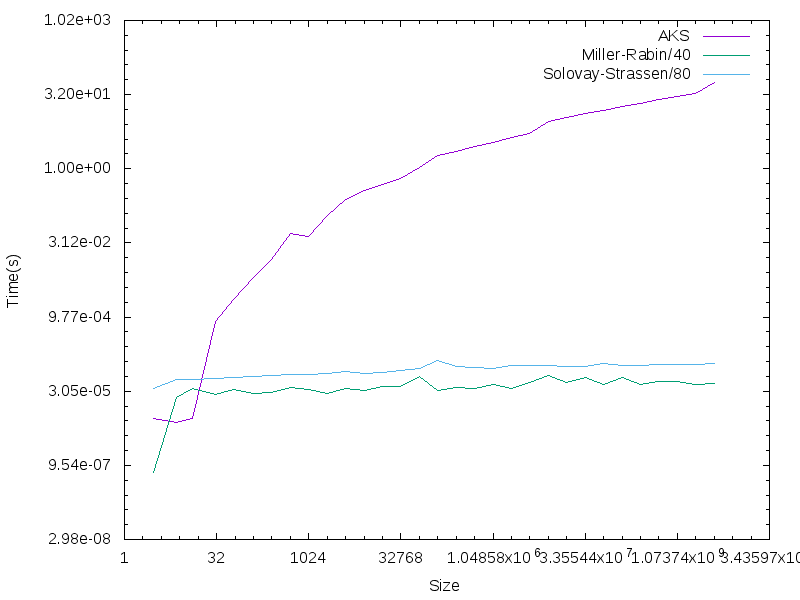
\includegraphics[totalheight=12cm]{img/graphs/aks-probs-primes-mean}
	\caption{Comparación AKS, Miller-Rabin/40 y Solovay-Strassen/80 con números primos}
\end{figure}

Como podemos comprobar, para entradas pequeñas, el algoritmo \textbf{AKS} funciona muy bien e, incluso, superando a los dos test probabilísticos. Sin embargo, vemos que entorno a $32 = 2^5$, el tiempo de ejecución se dispara, lo cual deja claro lo ineficiente del test \textbf{AKS}.\\

El test de \textit{Solovay-Strassen} es un poco peor que el de \textit{Miller-Rabin} porque realizamos el doble de rondas para asegurar probabilidades similares.\\

En conclusión, los tests probabilísticos funcionan mucho más rápido, lo cual es muy útil cuando estamos tratando con números muy grandes, además de que sus posibilidades de dar una respuesta errónea son prácticamente nulas debido a la cantidad de rondas.

\subsection{Potencias de Primos}

Puesto que el primer paso del test \textbf{AKS} es comprobar si la entrada es una potencia perfecta, es interesante ver cómo se comporta frente a los algoritmos probabilísticos con entradas que son potencias de primos.\\

Para esta comparación vamos a usar dos conjuntos distintos de prueba:

\begin{itemize}
	\item Potencias grandes de primos pequeños. En específico, primos de hasta $16$ bits elevados a $100$.
	
	\item Potencias pequeñas de primos grandes. En específico, primos de hasta $256$ bits elevados a $5$.
\end{itemize}

Primero empecemos con las potencias grandes de primos pequeños.

\begin{figure}[H]
	\centering
	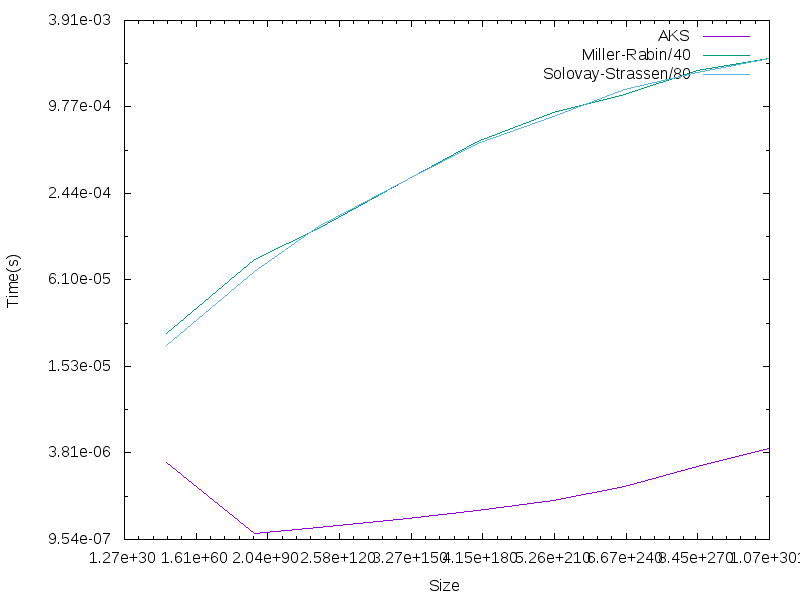
\includegraphics[totalheight=12cm]{img/graphs/aks-probs-powers-100-mean}
	\caption{Comparación AKS, Miller-Rabin/40 y Solovay-Strassen/80 con potencias grandes de primos pequeños}
\end{figure}

Y ahora la gráfica de potencias pequeñas de primos grandes.

\begin{figure}[H]
	\centering
	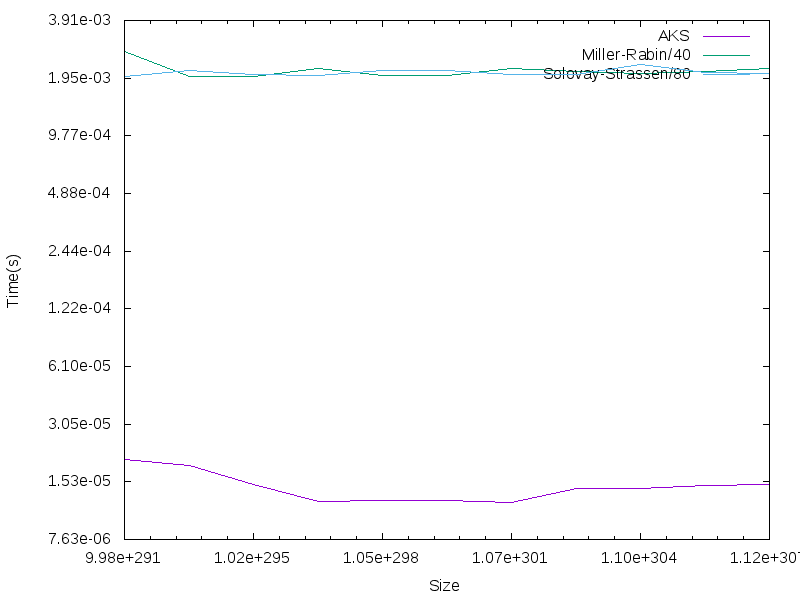
\includegraphics[totalheight=12cm]{img/graphs/aks-probs-powers-5-mean}
	\caption{Comparación AKS, Miller-Rabin/40 y Solovay-Strassen/80 con potencias pequeñas de primos grandes}
\end{figure}

En ambos casos, el análisis es claro. Comprobar si un número es una potencia perfecta es mucho más rápido que aplicar el test de \textit{Miller-Rabin} o el de \textit{Solovay-Strassen}.\\

Puesto que el test \textbf{AKS} maneja las potencias perfectas en el primer paso, y en vista de las gráficas anteriores, concluimos que el test \textbf{AKS} funciona mucho mejor que los test probabilísticos cuando la entrada se trata de una potencia perfecta.

\subsection{Números Compuestos No Potencias de Primos}

Habiendo hecho comparaciones con números primos y potencias de primos, es natural comparar usando números compuestos que no sean potencias de primos. Para ello usaremos números que son producto de dos o más factores primos grandes.\\

Esto nos ayudará a comprobar cómo se comportan los tres tests en los casos más sensibles, es decir, aquellos donde los factores primos son grandes. Determinar correctamente la composición de dichos números es de vital importancia en los protocolos de seguridad como RSA, pues de lo contrario, la seguridad de dicho sistemas se podría ver comprometida.\\

Usaremos distintos conjuntos de prueba:

\begin{itemize}
	\item Compuestos con factores primos grandes de magnitud similar. Por ejemplo, números compuestos que sean producto de un número de $256$ bits y $260$ bits.
	
	\item Compuestos con factores primos de magnitudes distintas. Por ejemplo, números compuestos con factores de $128$ bits y $256$ bits.
\end{itemize}

Vayamos con la gráfica del primer conjunto de prueba.

\begin{figure}[H]
	\centering
	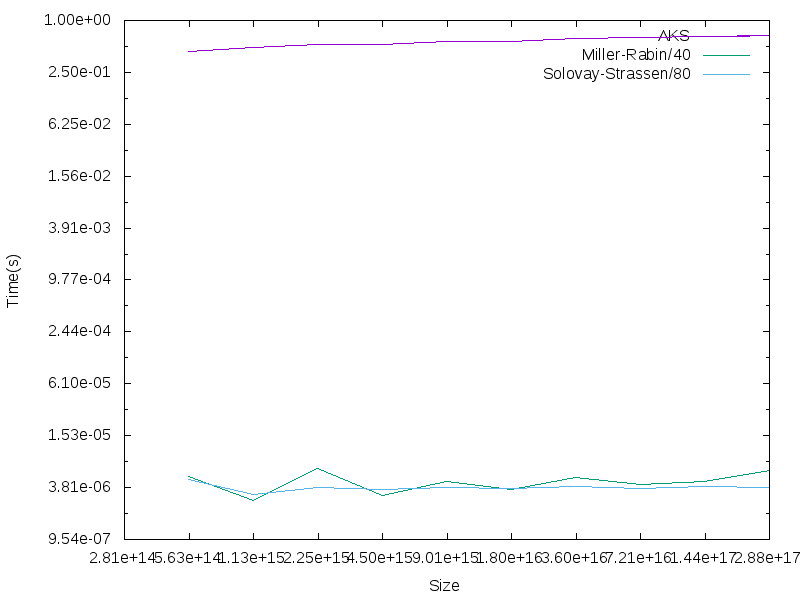
\includegraphics[totalheight=12cm]{img/graphs/aks-probs-comps-16-mean}
	\caption{Comparación AKS, Miller-Rabin/40 y Solovay-Strassen/80 con productos de primos de más de $32$ bits y otro de $16$ bits}
\end{figure}

Ahora veamos la gráfica del segundo.

\begin{figure}[H]
	\centering
	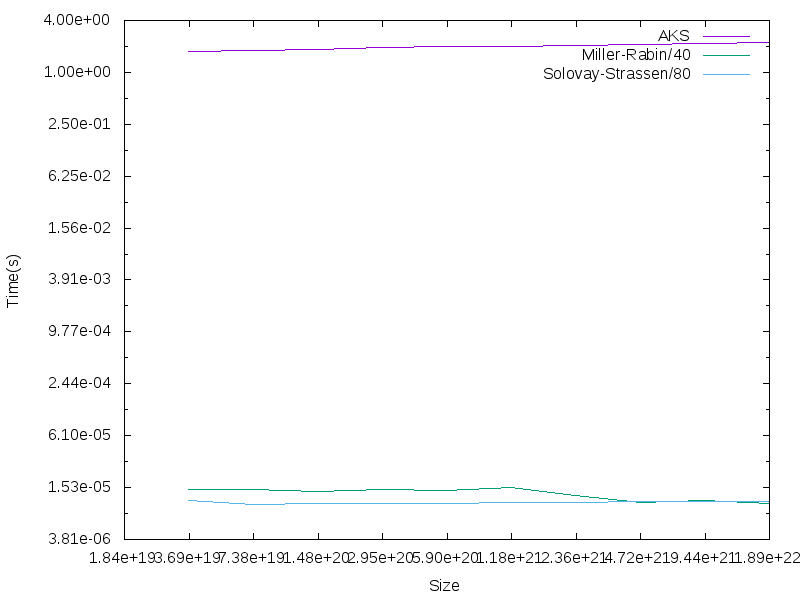
\includegraphics[totalheight=12cm]{img/graphs/aks-probs-comps-32-mean}
	\caption{Comparación AKS, Miller-Rabin/40 y Solovay-Strassen/80 con productos de primos de más de $32$ bits y otro de $32$ bits}
\end{figure}

Aparentemente, podemos comprobar que las gráficas son idénticas y que el tamaño de los factores no afecta en cómo se comportan el test \textbf{AKS} respecto de los otros.\\

Volvemos a comprobar, al igual que ya pasó con el caso en que la entrada eran primos, que el algoritmo \textbf{AKS} es bastante peor que sus contrapartes probabilísticas.

\section{Conclusión}

Como conclusión final de este apartado, y vistas las observaciones realizadas en esta comparación con los algoritmos probabilísticos, es que el algoritmo \textbf{AKS}, aún siendo general, polinómico, determinista e incondicional, es excesivamente lento para entradas no muy grandes, lo cual hace inviable su uso en otras aplicaciones de la criptografía.\\

Los algoritmos probabilísticos, aunque su respuesta no sea determinista, son suficientemente fiables en la mayoría de los casos, y su tiempo de ejecución los hace extremadamente convenientes cuando se trata de números con una gran cantidad de cifras.

\endinput
%------------------------------------------------------------------------------------
% FIN DEL CAPÍTULO. 
%------------------------------------------------------------------------------------
